\section{Технический проект}
\subsection{Общая характеристика организации решения задачи}

Программно-информационная система представляет собой современное веб-приложение, предназначенное для автоматизации управления книжным магазином. Система разработана с использованием модульной архитектуры, что позволяет легко адаптировать её к потребностям малого и среднего бизнеса, а также расширять функционал при необходимости.

В основе системы лежит серверная часть, реализованная на Flask с использованием RESTful API. Это обеспечивает быстрое и удобное взаимодействие между клиентской частью и сервером. Веб-интерфейс построен с использованием HTML, CSS и JavaScript, что делает систему доступной в любом современном браузере. База данных PostgreSQL выступает в качестве хранилища данных, а библиотека psycopg2 используется для взаимодействия с ней.

Система предоставляет удобные возможности для всех категорий пользователей. Покупатели могут просматривать каталог книг, использовать поиск, корзину для оформления заказов и отслеживать их статус. Также доступна страница книги с подробной информацией, включая описание и дополнительные характеристики.

Для сотрудников магазина предусмотрен интерфейс, позволяющий редактировать информацию о книгах, изменять их наличие, а также обновлять статусы заказов покупателей. Администраторы имеют доступ ко всему функционалу сотрудников, а также к управлению ролями пользователей. Это позволяет быстро изменять права доступа, добавлять новых сотрудников или ограничивать доступ к определённым функциям.

Система поддерживает аутентификацию и авторизацию пользователей, обеспечивая безопасное использование. Реализована возможность работы с несколькими ролями: покупатель, сотрудник и администратор, что делает её гибкой и подходящей для различных сценариев использования.

Ключевая особенность системы – её масштабируемость. Архитектура позволяет легко добавлять новые функции, такие как поддержка скидок, интеграция с платёжными системами или создание аналитических отчётов о продажах. Также предусмотрена возможность адаптации интерфейса под мобильные устройства, что обеспечивает доступность для пользователей с разных платформ.

Применение системы эффективно в книжных магазинах, где требуется централизованное управление ассортиментом и заказами. Её также можно модифицировать для других сфер розничной торговли. Перспективы развития включают добавление системы промокодов, расширение функционала аналитики и поддержку мультиязычного интерфейса, что сделает её полезным инструментом для международных пользователей.

Эта система сочетает простоту в использовании и высокую гибкость настройки, предоставляя удобные инструменты для управления книжным магазином.

\subsection{Обоснование выбора технологии проектирования}

Выбор технологий, языков программирования и архитектурных решений для реализации программно-информационной системы обусловлен совокупностью факторов, направленных на обеспечение высокой гибкости, надёжности и простоты сопровождения программного продукта. Используемые для создания программно-информационной системы языки и технологии отвечают современным практикам разработки, позволяют достичь высокой производительности и отказоустойчивости программы.

\subsubsection{Язык программирования Python}

В качестве языка программирования для серверной части выбран Python, благодаря его сочетанию выразительности, гибкости и обширной поддержки со стороны сообщества разработчиков. Python — это высокоуровневый, интерпретируемый язык, активно применяющийся как в образовательных, так и в промышленных проектах. Основные причины выбора языка заключаются в следующем:
\begin{enumerate}
	\item Простой и интуитивно понятный синтаксис значительно сокращает порог вхождения и снижает количество потенциальных ошибок при написании кода. Это особенно важно в условиях ограниченного времени на разработку и тестирование, а также при передаче проекта на сопровождение.
	\item Поддержка нескольких парадигм программирования, включая объектно-ориентированную, процедурную и функциональную, делает Python универсальным инструментом. Это позволяет организовать код в соответствии с принципами модульности, инкапсуляции и повторного использования.
	\item Обширная стандартная библиотека и внешняя экосистема обеспечивают доступ к готовым модулям для сериализации, построения интерфейса, анализа синтаксических деревьев, многопоточности и многого другого. Это существенно ускоряет разработку и упрощает реализацию сложных функций.
	\item Кроссплатформенность языка позволяет запускать приложение на операционных системах Windows, Linux и macOS без необходимости адаптации кода под конкретную платформу. Таким образом, обеспечивается максимальная универсальность и доступность системы для пользователя.	
\end{enumerate}


Таким образом, Python представляет собой оптимальное решение для реализации проекта, сочетающее в себе простоту, мощь и гибкость, что делает его незаменимым инструментом в учебных и практических задачах программной инженерии.

\subsubsection{Язык программирования JavaScript}
JavaScript выбран для клиентской части, так как он является основным языком для динамического взаимодействия в веб-приложениях. JavaScript исполняется непосредственно в браузере, обеспечивая интерактивность без необходимости перезагрузки страницы. Благодаря JavaScrpipt удалось реализовать следующее:
\begin{itemize}
	\item отправку асинхронных запросов к REST API для получения данных;
	\item динамическое обновление интерфейса;
	\item управление локальным хранилищем;
	\item обработку событий.
\end{itemize}
JavaScript обеспечивает событийно-ориентированную модель, что позволяет обрабатывать действия пользователя в реальном времени и интегрироваться с серверной частью через REST API.

\subsubsection{Интерфейс фреймворка Flask}
Flask -- это легковесный веб-фреймворк на основе Python, выбранный для реализации серверной части программно-информационной системы. Flask предоставляет минималистичный и гибкий интерфейс для создания RESTful API, что делает его подходящим для обработки HTTP-запросов и управления данными. Flask:

\begin{itemize}
	\item позволяет системе обрабатывать входящие HTTP-запросы для различных эндпоинтов;
	\item интегрируется с PostgreSQL через библиотеку psycopg2, что упрощает обработку данных на сервере и их передачу клиенту;
	\item позволяет обрабатывать исключения, возникающие при выполнении запросов.
\end{itemize}

Интерфейс Flask обеспечивает маршрутизацию запросов, управление сессиями и интеграцию с внешними библиотеками, что делает его удобным для реализации REST API.

Flask выбран благодаря своей простоте и способности эффективно решать задачи, связанные с созданием REST API. Легковесная архитектура минимизирует накладные расходы, обеспечивая быструю обработку запросов, что критично для веб-приложения с большим количеством пользователей.

\subsubsection{Графический интерфейс с использованием HTML и CSS}

HTML и CSS используются для создания структуры и оформления пользовательского интерфейса. HTML определяет разметку страниц. CSS задаёт стили, такие как цвета, шрифты, расположение элементов и адаптивность для разных устройств. Использование медиазапросов обеспечивает корректное отображение на компьютерах, планшетах и смартфонах. Разделение структуры и оформления упрощает поддержку и обновление интерфейса, обеспечивая интуитивно понятное взаимодействие для пользователей.

Выбор HTML и CSS обоснован их стандартизацией, простотой и способностью создавать адаптивный и функциональный интерфейс, соответствующий требованиям книжного магазина.

\subsection{Архитектура программной системы}

 Архитектура программно-информационной системы управления книжным магазином построена по клиент-серверной модели с использованием RESTful API для обеспечения взаимодействия между компонентами. Система состоит из трёх основных компонентов: клиентской части, серверной части и базы данных. На рисунке 3.1 представлена UML-диаграмма, иллюстрирующая архитектуру системы и взаимосвязи между её компонентами.

\begin{figure}[H]
	\centering
	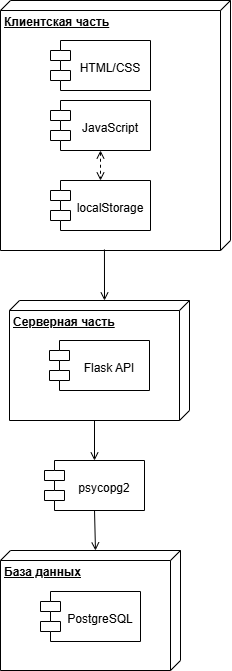
\includegraphics[width=0.3\linewidth]{images/диаграмма_компонентов}
	\caption{}
	\label{fig:}
\end{figure}


\subsubsection{Компоненты системы}

\paragraph{Клиентская часть}

Клиентская часть реализована как одностраничное веб-приложение, работающее в браузере пользователя. Используемые технологии включают HTML для разметки, CSS для стилизации и JavaScript для динамического взаимодействия. Основные функции клиентской части:
	\begin{enumerate}
		\item Отображение пользовательского интерфейса: каталог книг, корзина, панель администратора, модальные окна для авторизации, регистрации и просмотра деталей книг.
		\item Динамическое обновление данных: JavaScript использует Fetch API для асинхронных запросов к серверу, что позволяет обновлять содержимое страницы без перезагрузки.
		\item Хранение временных данных: используется localStorage для сохранения содержимого корзины и данных текущего пользователя. Это обеспечивает сохранение состояния приложения между сеансами.
		\item Обработка событий: JavaScript обрабатывает действия пользователя, такие как клики по кнопкам, ввод в поисковую строку или изменение количества товаров в корзине.
	\end{enumerate}
	
	Клиентская часть взаимодействует с сервером исключительно через REST API, отправляя HTTP-запросы и получая JSON-ответы.

\paragraph{Серверная часть}

Серверная часть реализована на Python с использованием фреймворка Flask. Сервер выступает в роли REST API, обеспечивая обработку запросов от клиента и взаимодействие с базой данных. Основные функции серверной части:
	\begin{enumerate}
		\item Маршрутизация запросов: Flask использует декораторы для определения эндпоинтов.
		\item Обработка данных: сервер принимает JSON-данные из POST-запросов или параметры строки запроса. Данные валидируются, обрабатываются и передаются в SQL-запросы к базе данных.
		\item Формирование ответов: сервер возвращает JSON-ответы, используя JSONEncoder для сериализации данных. Ответы включают данные или сообщения об ошибках с соответствующими HTTP-кодами.
		\item Интеграция с базой данных: сервер использует библиотеку psycopg2 для взаимодействия с PostgreSQL. Функция устанавливает соединение с базой данных для возврата результатов SQL-запросов в виде словарей.
		\item Обработка ошибок: в случае ошибок сервер откатывает транзакцию и возвращает JSON-ответ с описанием ошибки.
	\end{enumerate}

\paragraph{База данных}

База данных: реализована на PostgreSQL, которая хранит данные о книгах, авторах, жанрах, пользователях, заказах и элементах заказов. Основные аспекты:
	\begin{enumerate}
		\item Структура данных: база данных включает таблицы, которые связаны через внешние ключи.
		\item Доступ к данным: сервер выполняет SQL-запросы через psycopg2 для операций.
	\end{enumerate}
	
	PostgreSQL обеспечивает надёжное хранение данных и поддержку сложных запросов, таких как фильтрация книг по жанрам или авторам.

\subsection{Проект данных программной системы}

В программной системе книжного магазина используется реляционная СУБД PostgreSQL. Для взаимодействия с базой из Python-приложения применяется библиотека psycopg2.

На клиентской стороне используется localStorage для временного хранения данных корзины и информации о пользователе, что обеспечивает сохранение состояния без синхронизации с сервером.

На рисунке 3.2 представлена модель базы данных

\begin{figure}[H]
	\centering
	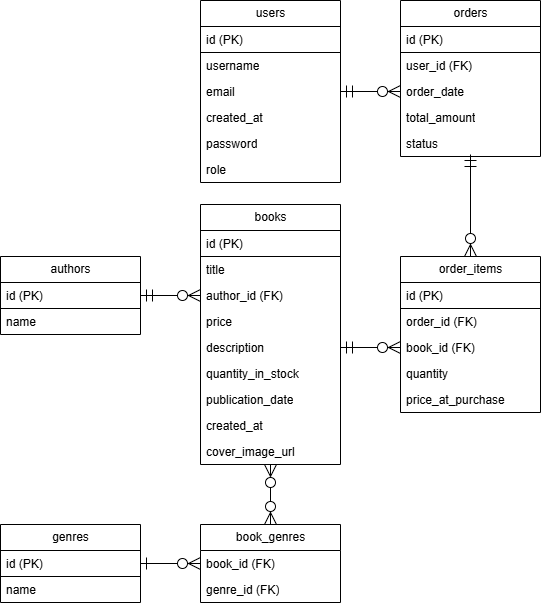
\includegraphics[width=0.7\linewidth]{images/концептуальная_модель}
	\caption{Модель базы данных}
	\label{fig:}
\end{figure}


\subsubsection{Описание сущностей}

 В таблице 3.1 приведен набор полей JSON-документа и их описание для сущности «Авторы».

\begin{xltabular}{\textwidth}{|c|c|X|}
	\caption{Описание сущности "Авторы"\label{authors:table}}\\ \hline
	\thead{Ключ} & \thead{Тип} & \thead{Описание} \\ \hline
	\endfirsthead
	\continuecaption{Продолжение таблицы \ref{authors:table}}\\ \hline
	\thead{Ключ} & \thead{Тип} & \thead{Описание} \\ \hline
	\endhead
	id & integer & Уникальный идентификатор автора (первичный ключ) \\ \hline
	name & varchar(100) & Полное имя автора \\ \hline
\end{xltabular}

 В таблице 3.2 приведен набор полей JSON-документа и их описание для сущности «Жанры».
 
\begin{xltabular}{\textwidth}{|c|c|X|}
	\caption{Описание сущности "Жанры"\label{genres:table}}\\ \hline
	\thead{Ключ} & \thead{Тип} & \thead{Описание} \\ \hline
	\endfirsthead
	\continuecaption{Продолжение таблицы \ref{genres:table}}\\ \hline
	\thead{Ключ} & \thead{Тип} & \thead{Описание} \\ \hline
	\endhead
	id & integer & Уникальный идентификатор жанра (первичный ключ) \\ \hline
	name & varchar(50) & Название жанра (уникальное) \\ \hline
\end{xltabular}

 В таблице 3.3 приведен набор полей JSON-документа и их описание для сущности «Книги».
 
\begin{xltabular}{\textwidth}{|c|c|X|}
	\caption{Описание сущности "Книги"\label{books:table}} \\ \hline
	\thead{Ключ} & \thead{Тип} & \thead{Описание} \\ \hline
	\endfirsthead
	\caption*{Продолжение таблицы \ref{books:table}} \\ \hline
	\thead{Ключ} & \thead{Тип} & \thead{Описание} \\ \hline
	\endhead
	id & integer & Уникальный идентификатор книги (первичный ключ) \\ \hline
	title & varchar(200) & Название книги \\ \hline
	author\_id & integer & Внешний ключ, ссылается на таблицу авторов \\ \hline
	genre\_id & integer & Внешний ключ, ссылается на таблицу жанров \\ \hline
	price & numeric(10,2) & Цена книги \\ \hline
	description & text & Описание книги (может быть NULL) \\ \hline
	quantity\_in\_stock & integer & Количество экземпляров на складе \\ \hline
	sold\_copies & integer & Количество проданных экземпляров \\ \hline
	publication\_date & date & Дата публикации (может быть NULL) \\ \hline
	created\_at & timestamp & Дата и время добавления книги \\ \hline
\end{xltabular}

 В таблице 3.4 приведен набор полей JSON-документа и их описание для сущности «Пользователи».
 
\begin{xltabular}{\textwidth}{|c|c|X|}
	\caption{Описание сущности "Пользователи"\label{users:table}}\\ \hline
	\thead{Ключ} & \thead{Тип} & \thead{Описание} \\ \hline
	\endfirsthead
	\continuecaption{Продолжение таблицы \ref{users:table}}\\ \hline
	\thead{Ключ} & \thead{Тип} & \thead{Описание} \\ \hline
	\endhead
	id & integer & Уникальный идентификатор пользователя (первичный ключ) \\ \hline
	username & varchar(50) & Логин пользователя (уникальный) \\ \hline
	email & varchar(100) & Email пользователя (уникальный, может быть NULL) \\ \hline
	password & text & Пароль пользователя \\ \hline
	role & varchar(20) & Роль: customer, employee, admin \\ \hline
	created\_at & timestamp & Дата и время регистрации \\ \hline
\end{xltabular}

 В таблице 3.5 приведен набор полей JSON-документа и их описание для сущности «Заказы».
 
\begin{xltabular}{\textwidth}{|c|c|X|}
	\caption{Описание сущности "Заказы"\label{orders:table}} \\ \hline
	\thead{Ключ} & \thead{Тип} & \thead{Описание} \\ \hline
	\endfirsthead
	
	\caption*{Продолжение таблицы \ref{orders:table}} \\ \hline
	\thead{Ключ} & \thead{Тип} & \thead{Описание} \\ \hline
	\endhead
	
	id & integer & Уникальный идентификатор заказа (первичный ключ) \\ \hline
	user\_id & integer & Внешний ключ, ссылается на таблицу пользователей \\ \hline
	order\_date & timestamp & Дата и время оформления заказа \\ \hline
	total\_amount & numeric(10,2) & Общая сумма заказа \\ \hline
	status & varchar(20) & Статус: processing, shipped, delivered, cancelled \\ \hline
\end{xltabular}
 В таблице 3.6 приведен набор полей JSON-документа и их описание для сущности «Элементы заказа».
 
\begin{xltabular}{\textwidth}{|c|c|X|}
	\caption{Описание сущности "Элементы заказа"\label{order_items:table}}\\ \hline
	\thead{Ключ} & \thead{Тип} & \thead{Описание} \\ \hline
	\endfirsthead
	\continuecaption{Продолжение таблицы \ref{order_items:table}}\\ \hline
	\thead{Ключ} & \thead{Тип} & \thead{Описание} \\ \hline
	\endhead
	id & integer & Уникальный идентификатор элемента заказа (первичный ключ) \\ \hline
	order\_id & integer & Внешний ключ, ссылается на таблицу заказов \\ \hline
	book\_id & integer & Внешний ключ, ссылается на таблицу книг \\ \hline
	quantity & integer & Количество экземпляров книги в заказе \\ \hline
	price\_at\_purchase & numeric(10,2) & Цена книги на момент покупки \\ \hline
\end{xltabular}

\subsection{Проектирование пользовательского интерфейса}

На основании требований к пользовательскому интерфейсу, представленных в пункте 2.3.3 технического задания, был разработан графический интерфейс программно-информационной системы управления книжным магазином. Для создания пользовательского интерфейса используется разметка, основанная на HTML и CSS.

На рисунке 3.1 представлен макет интерфейса главной страницы. Макет содержит следующие элементы:
\begin{enumerate}
	\item Поисковая строка.
	\item Карточка книги.
	\item Название книги.
	\item Автор книги.
	\item Цена книги.
	\item Количество на складе.
	\item Кнопка открывающая модальное окно с  подробным описанием книги.
	\item Кнопка добавляющая выбранную книгу в корзину.
	\item Кнопка открывающая модальное окно с авторизацией и регистрацией.
	\item Пагинация.
\end{enumerate}

\begin{figure}[H]
	\centering
	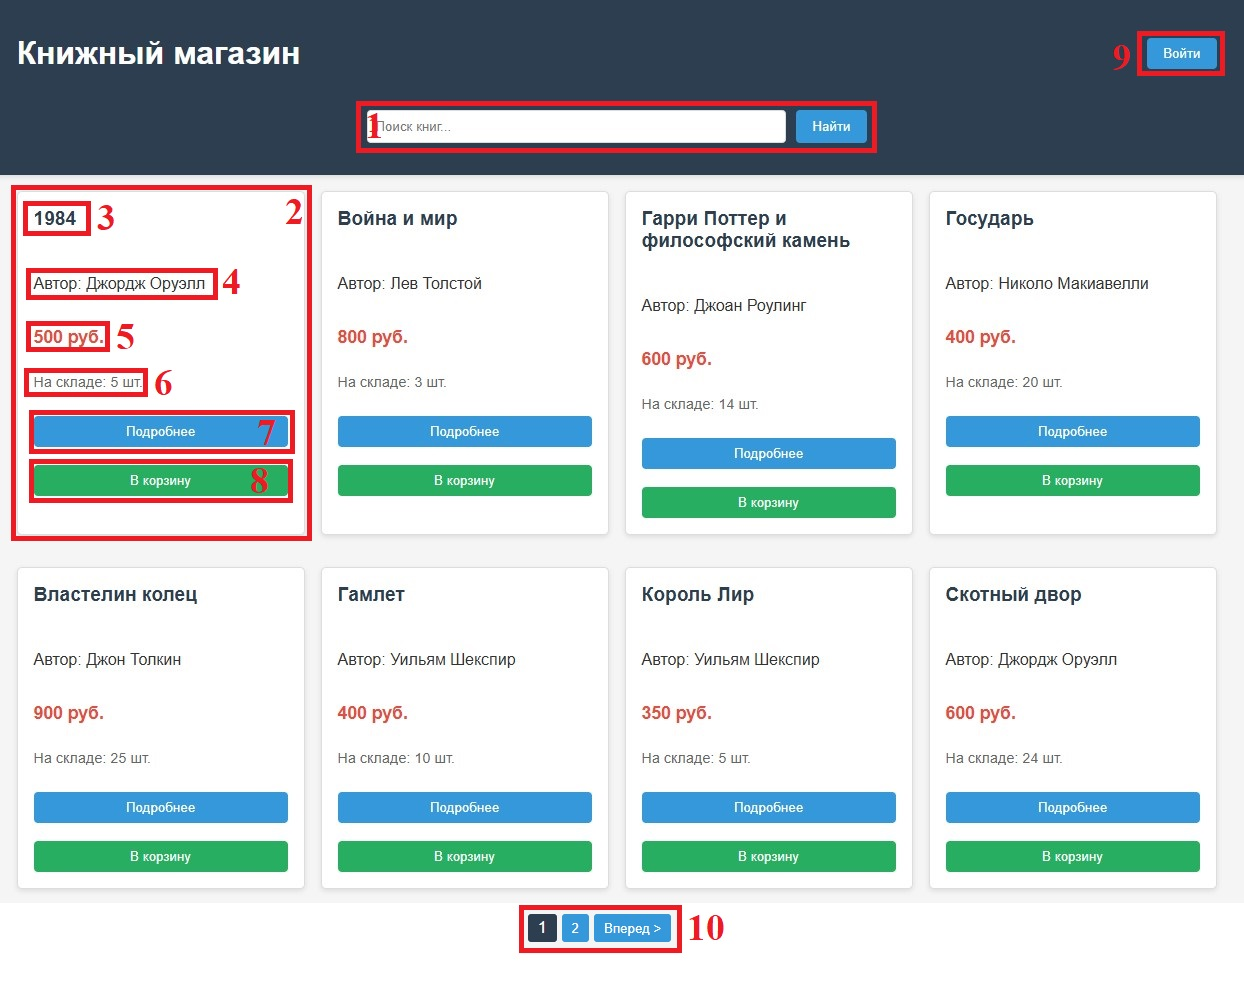
\includegraphics[width=0.7\linewidth]{images/Главная_страница}
	\caption{Макет интерфейса главной страницы}
	\label{fig:}
\end{figure}

На рисунке 3.2 представлен макет интерфейса корзины. Макет содержит следующие элементы:

\begin{enumerate}
	\item Книга добавленная пользователем в корзину.
	\item Количество и кнопки для изменения количества конкретной книги в корзине.
	\item Наименование книги.
	\item Суммарная стоимость выбранного количества книг одного наименования.
	\item Кнопка удаления книг одного наименования из корзины.
	\item Кнопка для оформления заказа.
	\item Итоговая стоимость книг в корзине.
\end{enumerate}

\begin{figure}[H]
	\centering
	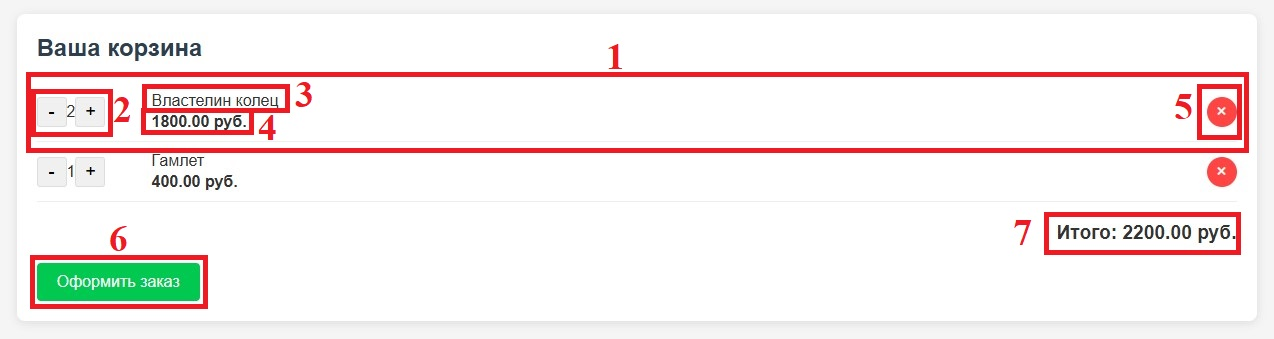
\includegraphics[width=0.7\linewidth]{images/Корзина}
	\caption{Макет интерфейса корзины}
	\label{fig:}
\end{figure}

На рисунке 3.3 представлен макет панели администратора. Макет содержит следующие элементы:

\begin{enumerate}
	\item Поле ввода для имени пользователя.
	\item Выпадающий список с выбором роли.
	\item Кнопка применения роли для выбраного пользователя.
	\item Кнопка актуализации данных списка пользователей.
	\item Список всех учётных записей и их данных.
	\item Кнопка для перехода к форме добавления книги.
\end{enumerate}

\begin{figure}[H]
	\centering
	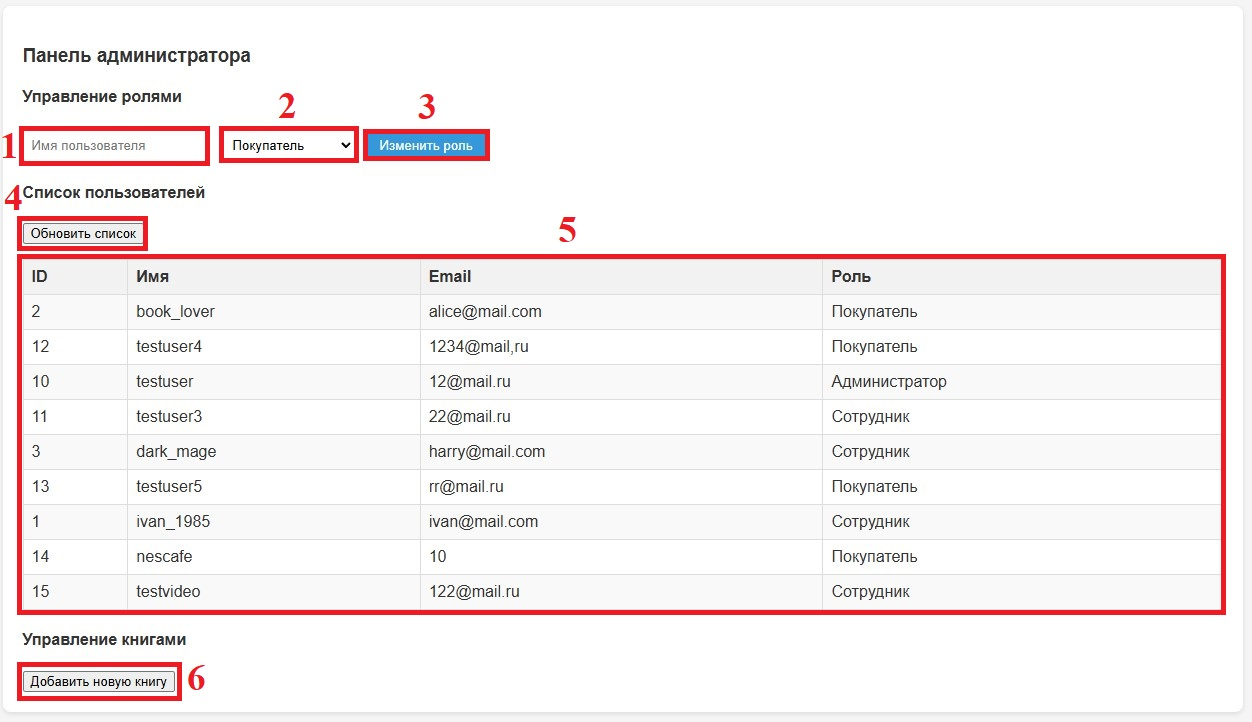
\includegraphics[width=0.7\linewidth]{images/Панель_администратора}
	\caption{Макет интерфейса панели администратора}
	\label{fig:}
\end{figure}

